%A Nikon F bajonett a modern SLR és DSLR fényképezőgépek által használt objektívcsatlakozás, amely tartalmaz mechanikus elemeket, valamint tartalmazhat elektronikus csatlakozásokat is.

"Nikon SLR-eken és NIKKOR objektíveken, a Nikon F 1959-es bemutatásától a mai modellekig használatos bajonett típusú F-csatlakozás egy kommunikációs kapcsolat Nikon SLR-ek és Nikon objektívek között.

Erős felépítéséről és kiemelkedő megbízhatóságáról emlékezetessé vált, az F-Csatlakozás kiemelkedő a NIKKOR objektívekkel való magasfokú kompatibilitásnak és egy olyan dizájnnak köszönhetően, amely képes magába foglalni későbbi fejlődéseket. A Nikon fenntartotta a csatlakozás alap struktúráját az 50 éven át tartó használata során, és jelenleg nagyjából 400 különböző objektív kompatibilis a rendszerrel. A Nikon F-Csatlakozás egyik legnagyobb előnye, hogy lehet egy nagy objektívkollekcióból választani, amibe beletartoznak az AF NIKKOR, AF-S (Silent Wave Motor) és PC-E perspective-control (perspektíva kontroll) NIKKOR objektívek is.

Az F-Csatlakozás és a NIKKOR objektívek képességeinek adaptálásával és bővítésével, Nikon beépített technológiákat, mint például autófókusz, fejlett fénymérés, távolság információ technológia, elektronikus rekeszátmérő irányítás a G-típusú NIKKOR-ban, VR (Vibráció Redukció) képstabilizálás és Silent Wave Motor (AF-S), ezáltal fenntartva egy jelentős fokú kompatibilitást, ezzel demonstrálva egy folyamatos elköteleződést o fényképészek iránt."\cite{Nikon_F_mount-ról}

%Used on Nikon SLRs and NIKKOR lenses from the introduction of the Nikon F in 1959 to current models, the bayonet-type F-Mount is the communication link between Nikon SLRs and NIKKOR lenses.

%"Noted for its rugged construction and outstanding reliability, the F-Mount is distinctive also for its degree of compatibility with NIKKOR lenses and a design that can accommodate future system advances. Nikon has maintained the basic structure of the mount for the 50 years of its use, and currently some 400 different NIKKOR lenses are compatible with the system.
%One of the biggest advantages of the Nikon F-Mount is that you're able to choose from a large selection of lenses including: AF NIKKOR and AF-S (Silent Wave Motor) and PC-E perspective-control NIKKOR lenses.

%By adapting and extending the capability of the F-Mount and NIKKOR lenses, Nikon has incorporated technologies like autofocus, advanced metering, distance information technology, electronic aperture control in G-Type NIKKOR, VR (Vibration Reduction) image stabilization and Silent Wave Motor (AF-S) technology, thus maintaining a significant degree of compatibility and demonstrating an ongoing commitment to photographers."

\paragraph{Felépítése}

%IDE KELL EGY RÖID ISMERTETÉS A CSATLAKOZÁS RÖGZÍTÉSÉRŐL
"(...) egy F-csatlakozás nem egy menetes csatlakozás; hanem, egy bajonett csatlakozás. A bajonett csatlakozások nagyon jók fényképezéshez, mivel álataluk a kamera felhasználója könnyeb és hatékonyan tud objektíveket különböző körülményekhez cserélni, és könnyen integrálhatóvá teszik az elektronikus funkciókat (írisz/fókusz irányítás), mivel ezek kiszémítható, pontos mechanizmusok."\cite{Nikon-bajonett}
%an F-mount is not a threaded mount; rather, it is a bayonet
%mount. Bayonet mounts are great
%for photography, as they allow the
%user of the camera to swap lenses
%out quickly and efficiently for different scenarios, and allows for the
%easy integration of electronic features (iris/focus control) since they
%are a clocked mechanism.
\paragraph{Rögzítés}
A csatlakozás felettébb tartós\cite{Nikon_F_mount-ról}.
Az objektívet az azon és a fénykpezővázon feltüntetett jelzések mentén kell a váz csatlakozójára illeszteni, majd elforgatni.
A megfelelő illesztés során az objektív csatlakozója enyhén belecsúszik a vázoldali részbe, ahol a kettő gyűrűjének a kialakítása vezeti az objektívet a forgatás során.
A túl, vagy rossz irányú forgatást ütközők akadályozzák meg.
Amikor az objektív a megfelelő pozícióba ér, egy rugó által kitolt tüske rögzíti azt.
Levételkor egy gomb elnyomásának, vagy egy rugós kapcsoló elhúzásának köszönhetően ez a tüske visszahúzódik, így engedélyezve az objektív levehető pozíció felé mozgatását.

\paragraph{Kommunikáció}
A Nikon F bajonettcsatlakozónál az objektív és a fényképezőgépváz közötti kommunikáció történhet mechanikai(AI, AI-S jelölésű objektívek)\cite{Lens_naming}, elektronikai (E jelölésű objektívek)\cite{Lens_naming}, valamint egyszerre mechanikai és elektronikai (AI-P, AF, AF-I, D és G jelölésű objektívek)%\cite{Nikon_naming_convention}
\cite{Nikon_CPU}úton. Ezeken a kategóriákon belüli csatlakozók között lehetnek további különbségek az eszközök funkcióitól függően.

\subsection{Objektív oldali csatlakozó}

\subsubsection{Elektrnikus kommunikáció:}
UPDATE WITH NIKON HACKERS STUFF. REFERENCE REPAIR MANUALS FOR THE CONTACTS. ADD KNOWN PROTOCOL CODES.
Az összes CPU-val rendelkező objektív csatlakozásán találhatóak elektronikus kontaktok \cite{Nikon_CPU}. Ezek feladata az, hogy gyors kommunikációt létesítsenek az objektív és a kameraváz között.
A kamera által az objektívvel elektronikusan közölt információk:
\begin{itemize}
    \item Amennyiben az objektív nem AF típusú autófókuszmechanizmust tartalmaz, a fókuszáláshoz szükséges adatok.
    \item E jelölésű objektíveknél rekeszátmérőt állító jelek.
\end{itemize}
Ezeken kívül a kamera elelektromos árammal is ellátja ezeket az eszközöket, ezzel biztosítva azt, hogy az objektívek és kiegészítők megfelelően, külső áramforrás nélkül tudjanak üzemelni. A CPU kontaktok száma objektívek között váltózó.\cite{Nikon_CPU} AF-I, AF-S és AF-P esetében a beépített fókuszmotornak is ez szolgál áramforrásként.

%Ez itt a \ref{fig:AF_kontakt} ábra.
\begin{figure}[H]
	\centering
	\includegraphics[width=0.5\linewidth]{img/Nikon_50mm_1.8_kontaktok.jpg}
	\caption{Elektronikus kontaktok Nikon AF típusú objektíven}
	\label{fig:AF_kontakt}
\end{figure}

\begin{figure}[H]
	\centering
	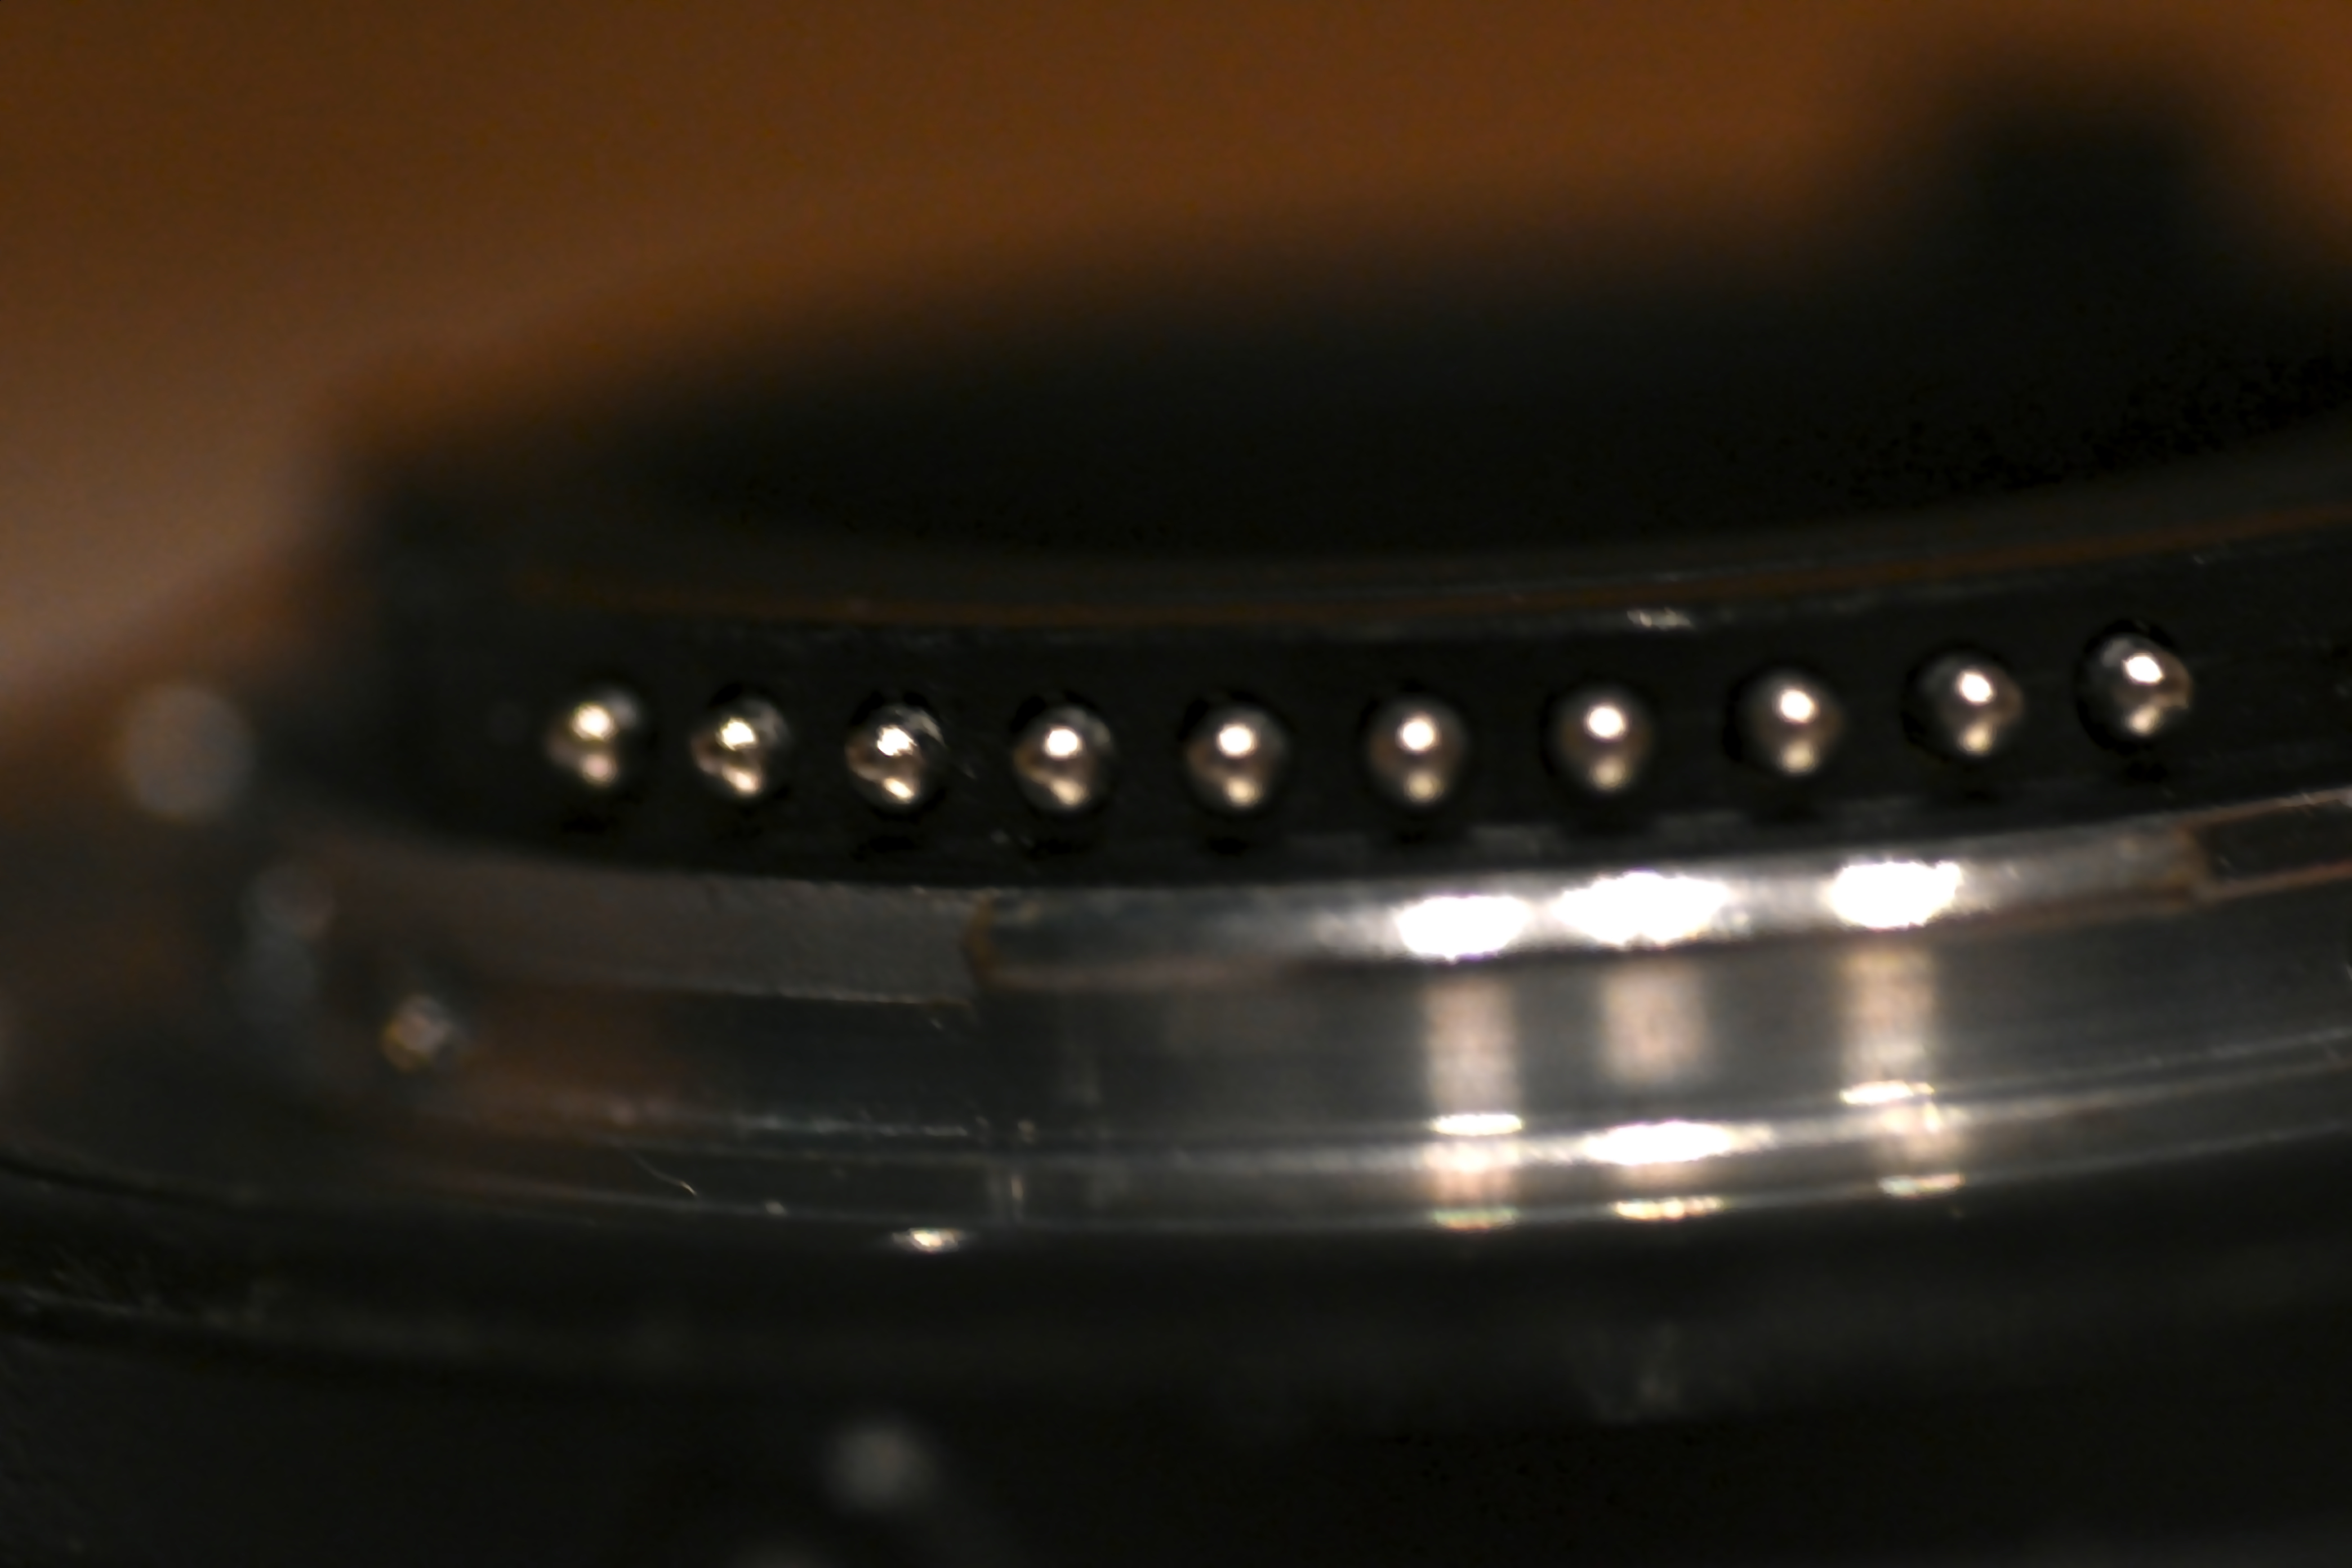
\includegraphics[width=0.5\linewidth]{img/Nikon_17-55_kontaktok.jpg}
	\caption{Elektronikus kontaktok Nikon AF-S DX 17-55mm f/2.8 G objektíven}
	\label{fig:G_kontakt}
\end{figure}

% \begin{figure}[H]
% 	\centering
% 	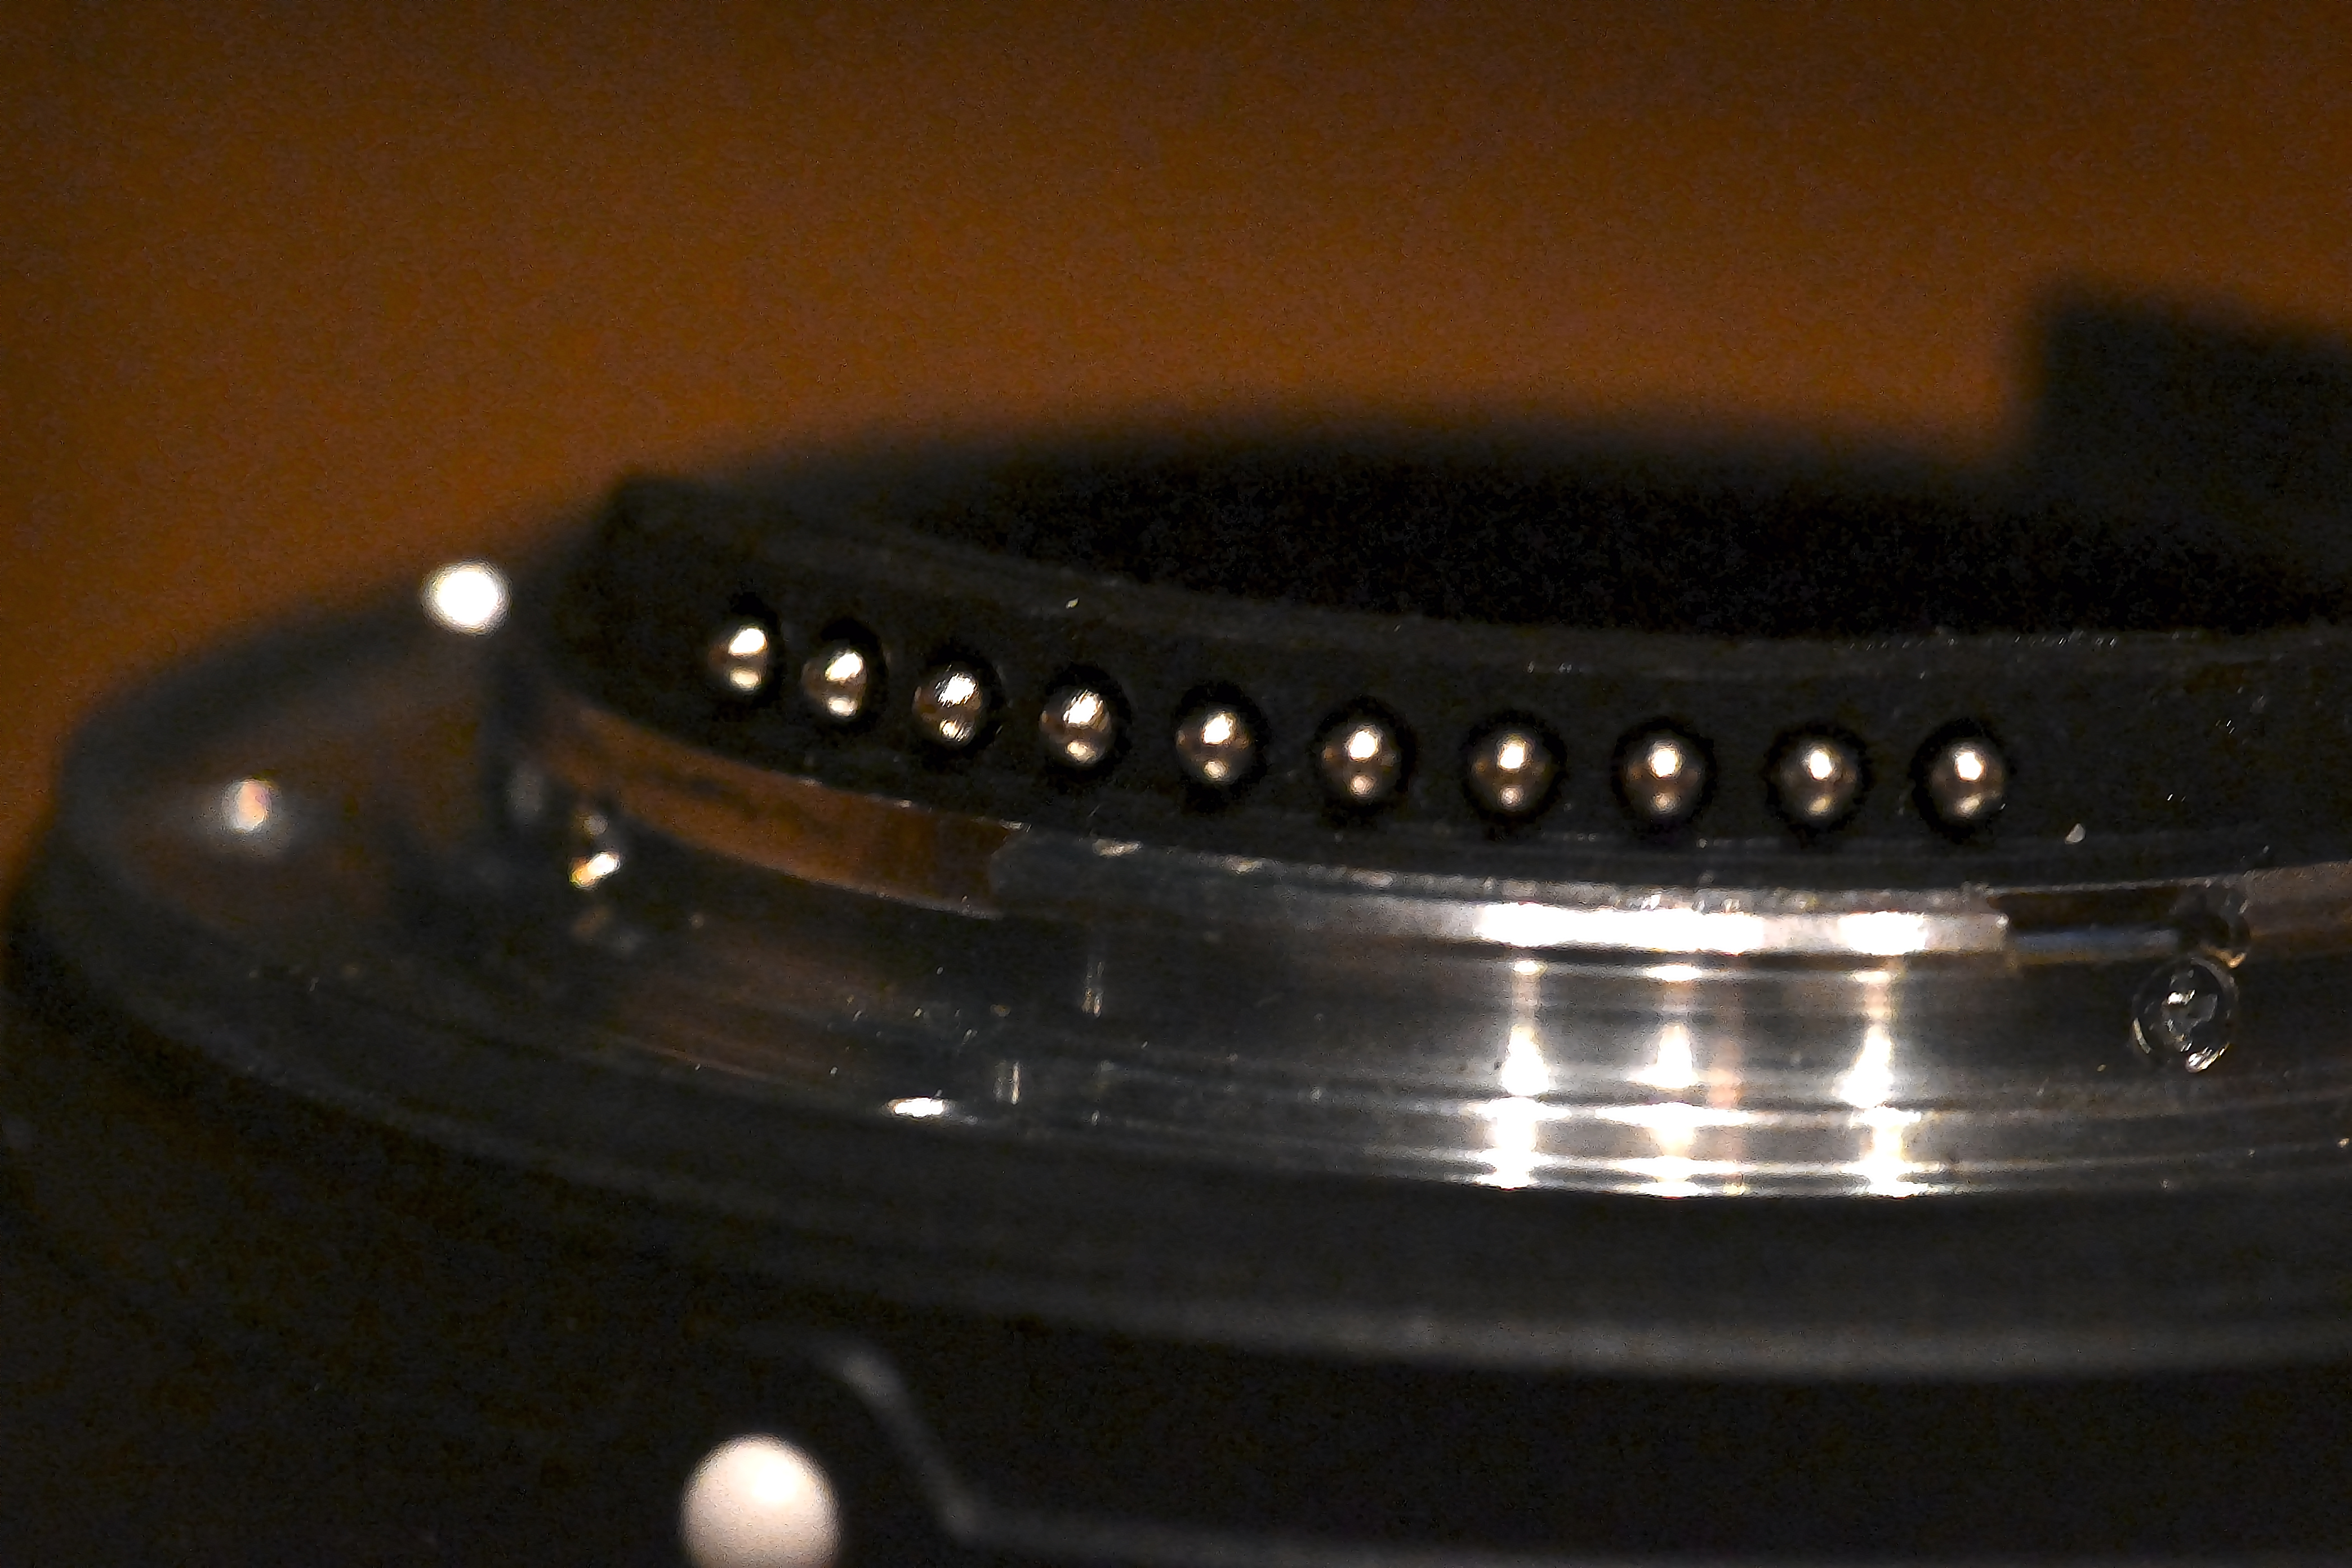
\includegraphics[width=0.5\linewidth]{img/Nikon_70-200E_kontaktok.jpg}
% 	\caption{Elektronikus kontaktok Nikon AF-S 70-200mm E FL ED VR objektíven}
% 	\label{fig:E_kontakt}
% \end{figure}

\subsubsection{Mechanikus kommunikáció}
A CPU-val nem rendelkező objektívek nem tudnak elektronikus úton kommunikálni, ezért a kommunikáció jelentős mértékben lekorlátozódik, és csak kevés információ, lassú cseréje lehetséges. Ennek ellenére a visszafelé kompatibilitás megőrzése érdekében és a technológia egyszerűségének köszönhetően, az E jelölésű objektíveken kívűl minden objektív rendelkezik ilyen kapcsolatokkal.
A fényképezőváz által az objektíveken mechanikusan állított értékek:
\begin{itemize}
    \item AF objektívek esetén fókusztávolság. [\ref{fig:AF_csavar}]
    \begin{figure}[H]
    	\centering
    	\includegraphics[width=0.5\linewidth]{img/Nikon_50mm_1.8_AF_csavar.jpg}
    	\caption{Fókuszállító csavar Nikon AF típusú objektíven}
    	\label{fig:AF_csavar}
    \end{figure}
    \item Rekeszátmérő (Az E jelölésű objektívek kivételével).
    \begin{itemize}
        \item Nyílt vagy zárt pozíció \ref{fig:G_rekeszkar}
        \begin{figure}[H]
        	\centering
        	\includegraphics[width=0.5\linewidth]{img/Nikon_17-55_rekeszkar.jpg}
        	\caption{Mechanikus kar a rekesz nyitására és zárására használt álláskapcsoló G típusú Nikon objektíven}
        	\label{fig:G_rekeszkar}
        \end{figure}
        \item Jelenleg beállított érték\ref{fig:Exposure_coupleing}
        \begin{figure}[H]
        	\centering
        	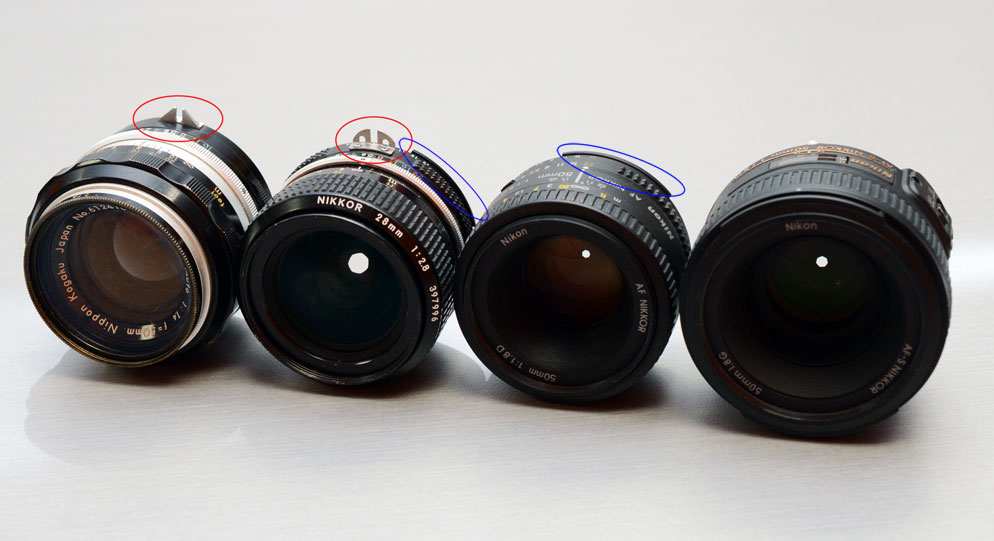
\includegraphics[width=0.75\linewidth]{img/lenses-AI-and-non-AI.jpg}
        	\caption{Nikon objektívek mechanikus rekeszátmérő csatlakozói \cite{Legacy_lenses}}
            \medskip
            \Centering
            \small Balról jobbra: Nikon AI-elötti objektív, rekeszátmérő csatlakozó cipő pirossal bekarikázva; Nikon AI objektív,  rekeszátmérő csatlakozó cipő pirossal bekarikázva, rekeszátmérő csatlakozó gerinc kékkel bekarikázva; Nikon AF-D objektív, rekeszátmérő csatlakozó gerinc kékkel bekarikázva; Nikon AF-S objektív nem kommunikál rekeszátmérő információt mechanikusan.\cite{Legacy_lenses}
        	\label{fig:Exposure_coupleing}
        \end{figure}
    \end{itemize}
\end{itemize}

\subsubsection{Rekeszátmérő állítás}
A fényképezés során legtöbb esetben a fókuszálást nem a kiválasztott rekeszértékkel végzi a kamera (autómatikusan) vagy a fényképész (manuálisan). Emmiatt a rekeszértéket a fénykép készítése elött a megfelelő értékre kell állítani. Ez régebbi objektíveknél manuálisan történt (ezek nem használhatóak a modern SLR és DSLR rendszerekkel), de az F bajonettes objektíveknél ez már autómatikusan az "autómatikus diafragmánaknak" köszönhetően valósul meg. Ilyenkor amennyiben a rekeszátmérő nem esik egy előre meghatározott érték alá, a fókuszáláskor használatos rekeszátmérő megegyezik a kép készítésekor felvett rekeszátmérővel. Ellenkező esetben a fénykép készítésekor a diafragma a nyilt (\ref{fig:17-55_nyilt} ábra) állásáról a zárt (\ref{fig:17-55_zart} ábra) állására ugrik át, ami már a beállított érték. Ennek a folyamatnak minél gyorsabbnak kell lennie, hogy a fényképen az látszódjon, amit a kezelő a gomb lenyomásakor beállított. \cite{Practical_design_considerations_for_modern_photographic_optics}
\paragraph{Kívánt érték megadása}
A kívánatos érték érték a Nikon rendszereken kettő féle képpen történhet meg:
\begin{itemize}
    \item Objektíven a rekeszátmérő gyűrű segítségével.(G és E objektíveken nem elérhető)
    \item A kamerán lávő rekeszátmérő állító kerékkel.
\end{itemize}
Amennyiben az objektív mindkét lehetőséget használatát megengedi, a vázon a fényképésznek be kell állítania, hogy melyik módszert szándékozik használni. Amennyiben a fényképezőgépen akarja állítani az értéket, egy rekeszátmérő gyűrűvel rendelkező objektív használatánál, a rekeszátmérőt az objektíven található gyűrűn a legnagyobb f-értékre kell állítania a felhasználónak. Erre a lépésre fényképezőgép is figyelmeztet.\cite{Nikon_D6_referencia_használati_utasítás}

\paragraph{Mechanikus autómatikus diafragma}
A legtöbb Nikon objektíven ilyen autómatikus diafrámmal rendelkezik. A (\ref{fig:G_rekeszkar}) képen látható álláskapcsolót egy rugó (amennyiben a álláskapcsolót más meg nem mozdítja) a zárt pozíció felé tolja. A fókuszálás során a álláskapcsolót egy, a fényképezőgépvázon található kar, a nyílt pozícióba tolja. A kép készítésekor ez a kar úgy mozdul, mogy az álláskapcsoló szabadon a zárt pozícióba tudjom kerülni, a rugó nyomásának köszönhetően. Eközben a rekeszátmérőért felelős lamellák addig záródnak össze, amíg meg nem állítja őket az objektív belső mechanikája, ami a fényképkészítő gomb lenyomása elött került beállításra. Az álláskapcsoló addig marad zárt állásban, amíg a fényképezőgép kéri, ezt követően a kar visszaviszi a kapcsolót a nyílt állásba, és várja a további utasításokat. A zárt állapot több kép elkészítésén át is fennmaradhat, amennyiben azok elég nyorsan követik egymást. Az álláskapcsoló állása bináris, így vagy teljesen nyílt, vagy teljesen zárt állapotban van, a kettő között nem állítható be átmeneti állapot.

\paragraph{Elektronikus autómatikus diafragma}
Kizárólag E jelölésű objektívek használják ezt a módszer. "Egy elektromágneses diafragma mechanizmus van beépítve ezen objektívek testébe, amit elektromos jelek irányítanak a fényképezővázból. "\cite{Lens_naming}

\begin{figure}[H]
	\centering
	\includegraphics[width=0.5\linewidth]{img/Nikon_17-55_zart.jpg}
	\caption{Nyugalmi állapotban a G jelölésű objektív rekesze zárva van.}
	\label{fig:17-55_zart}
\end{figure}

\begin{figure}[H]
	\centering
	\includegraphics[width=0.5\linewidth]{img/Nikon_17-55_nyilt.jpg}
	\caption{A rekeszátmérő kart elhúzva a rekesz kinyílik.}
	\label{fig:17-55_nyilt}
\end{figure}

\paragraph{Csavar alapú autófókusz}

Az objektíveknél, amelyek ezt a mechanizmust használják, "nem lehet az autófókuszt üzemeltetni, kivéve ha egy beépített fókuszmotorral rendelkező digitális vagy film SLR kamera van használva." A fókuszálási sebesség attól függ, hogy a vázba épített fókuszmotor, milyen sebességgel képes forgatni a (\ref{fig:F100_AF_csavar}) képen látható csavarfejet, ami a (\ref{fig:AF_csavar}) képen látszódó csavart hajtja meg.
% there can be no autofocus operation unless a digital or film SLR camera with the autofocus motor built-in to the camera body is used

\subsection{Váz oldali csatlakozó}
\subsubsection{Elektronikus kommunikáció}
Az összes modern Nikon SLR és DSLR bajonettje rendelkezik elektronikus csatlakozókkal. Ezek a következő információkat kapják az objektívektől és kiegészítőtől elektronikus úton:
\begin{itemize}
    \item Az objektívet vagy kiegészítőt azonosító információ.
    \begin{itemize}
        \item Az objektív maximális rekeszátmérője.
        \item Az objektív minimális rekeszátmérője.
        \item Az objektív elnevezése.
        \item Az objektív gyújtótávolsága.%\cite{Nikon_naming_convention}
    \end{itemize}
    \item Az objektív jelenlegi rekeszátmérője.
    \item Az objektív autófókuszálásához szükséges információk.
    \item D, G és E jelölésű objektíveknél az objektíven beállított fókusztávolság.
    \item Egyéb fénymérést segítő információ.
\end{itemize}

\subsubsection{Mechanikus kommunikáció:}
%Az objektív által a fényképezőgépváznak mechanikusan csak az objektív gyújtótávolsága adható át, az is kizárólag AI típusú objektíveknél\ref{fig:Exposure_coupleing}.Ez csak a kevés filmes Nikon kamerával működik, és a legtöbb fényképezőgép nem nyeri ki ezt az információt ezen az úton.\cite{Nikon_CPU}\cite{Nikon_naming_convention}
A fényképezőgépvázak képesek limitált mechanikus kommunikációt létesíteni F-bajonettes objektívekkel. E során a következő információkat tudják kinyerni:
\begin{itemize}
    \item Objektív gyújtótűvolsága, AI-típusú objektíveken %\cite{Nikon_naming_convention}
    \item Objektív jelenleg beállított rekeszátmérője. \cite{Lens_naming}
    \item Objektív maximális rekeszátmérője. \cite{Lens_naming}
\end{itemize}
%\begin{figure}[H]
%	\centering
%	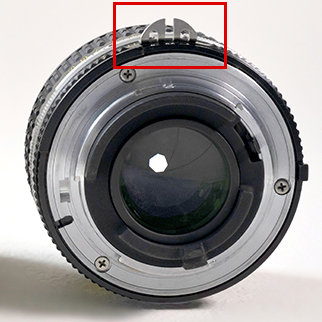
\includegraphics[width=0.5\linewidth]{img/Nikon-AI-bütyök.jpg}
%	\caption{Nikon AI objektív csatlakozása. Rekeszátmérő csatlakozó bekeretezve.\cite{Nikon_CPU}}
%	\label{fig:AI_back}
%\end{figure}

\begin{figure}[H]
	\centering
	\includegraphics[width=0.5\linewidth]{img/F100_bajonett.jpg}
	\caption{Nikon F100-as fényképezővázon található F bajonettcsatlakozás}
	\label{fig:F_bajonett}
\end{figure}

% \begin{figure}[H]
% 	\centering
% 	\includegraphics[width=0.5\linewidth]{img/F100_AF_csavar.jpg}
% 	\caption{Nikon fényképezőgépvázon található AF fókuszáló csavar}
% 	\label{fig:F100_AF_csavar}
% \end{figure}
%\paragraph{}